\documentclass{scrreprt}
\usepackage{listings}
\usepackage{graphicx}
\usepackage[toc,page]{appendix}
\usepackage[utf8]{inputenc}
\usepackage{caption}

\usepackage{listings}
%\usepackage{fontspec}
\DeclareFontShape{OT1}{cmtt}{bx}{n}{<5><6><7><8><9><10><10.95><12><14.4><17.28><20.74><24.88>cmttb10}{}

\author{Christophe Quignon}
\date{08. Apr. 2014}
\title{Artificial Intelligence for Robots}
\begin{document}
\maketitle
\section*{Both the performance measure and the utility function measure how well an agent is doing.
Explain the difference between the two.}
The performance measure indicates how successful an agent was. 
The utility function measure tells the agent which state the agent has to choose to achieve its goal.
The difference between these two is the time at which they take place. The utility function is predictive, the performance measure is descriptive.
%performance is more general, utility is more specific
\section*{What is a Braitenberg vehicle? How would you classify Braitenberg vehicles? Are they
reflex-, model-, goal-, or utility-based agents?}
The Braitenberg vehicle consists of at least two sensors which directly controll the wheels of the vehicle. Depending on the wiring, the Braitenberg vehicle is either attracted or opposed to the sensed input.\\
The Braitenberg vehicle has no internal states, no world model , no utilities and no abstract goal. Therefore, the Braitenberg vehicle is a reflex based agent.

\section*{Define in your own words the following terms: intelligence, artificial intelligence, state,
state space, search tree, search node, goal, action, successor function, and branching factor.}
\begin{itemize}
 \item  intelligence\\
 Intelligence is the ability to come up with sollutions to non-trivial problems.
 \item artificial intelligence\\
 Artificial intelligence is the aim to create engineer intelligence.
 \item state\\
 A state is a well defined, enclosed and stable position of a system.
 \item state space\\
 The state space contains all states of system.
 \item search tree\\
 A search tree is the complete description of every possible path from the beginning of initial position to every end position. The tree unfolds from the initial state and then recursivly connects all possible next stept.
 \item search node\\
 A search node is a state inside the search tree. It may also be a tree or a leaf of the search tree.
 \item goal\\
 A goal is the intended final position of a problem.
 \item action\\
 An action describes the procedure to change from one state to anoter.
 \item successor function\\
 The successor function of a node returns all subtrees of this node.
 \item branching factor\\
 The branching factor describes how many sucessors a node has.
\end{itemize}



\section*{[AIMA 3.6] Does a finite state space always lead to a finite search tree? How about a finite
state space that is a tree? Can you be more precise about what types of state spaces always lead to
finite search trees? (Adapted from Bender, 1996.)}
No, a finite search space does not have a finite search tree if it has circular successors. Nonetheless it has a search tree. But the tree may also be infinite. Non-circular search spaces always have a finite search tree.

\section*{[AIMA 3.9] The missionaries and cannibals problem is usually stated as follows. Three
missionaries and three cannibals are on one side of a river, along with a boat that can hold one or two
people. Find a way to get everyone to the other side, without ever leaving a group of missionaries
in one place outnumbered by the cannibals in that place. This problem is famous in AI because it
was the subject of the first paper that approached problem formulation from an analytical viewpoint
(Amarel, 1968).}
NOTE: The given solution wrongly discusses a similar problem where there is a guard on the boat which protects the missionaries on his side of the river bank.\\
Sorry for the mistake, but there was no time left fixing it.
\subsection*{Formulate the problem precisely, making only those distinctions necessary to ensure a valid
solution. Draw a diagram of the complete state space.}
\begin{figure}[hp]
  \centering
  \fbox{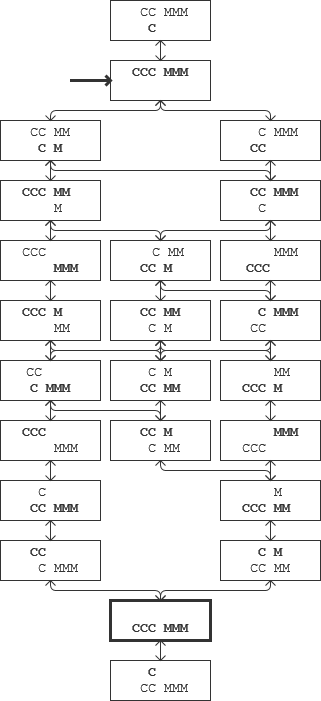
\includegraphics[width=70mm]{canibalen.png}} 
  \caption*{Search space of the missionaries (M) and cannibals (C) problem. The position of the boat is indicated in bold. The upper row is the starting riverside, the lower row is the desired riverside.}
  \label{}
\end{figure}
The problem is specified by the following restrictions:\\
\begin{lstlisting}
Every state consists of:
  two riversides R, 6 persons P and one boat B.

The two riversides are the start riverside s and the goal riverside g,   
R=(s, g)

The 6 persons are three cannibals c and three missionaries m:
P = (c, c, c, m, m, m)

R may contain:
   a subset of [P, b]

To change the state, the following conditions have to be met:
  The B must change from R to R' which is not R
  One or two P must change from R to R' which is not R
  For R without B holds:
    c < m OR m = 0

The initial state is:
S=[B, P]

The goal is:
G=[B, P] 
\end{lstlisting}  

\subsection*{Implement and solve the problem optimally using an appropriate search algorithm. Is it a good
idea to check for repeated states?}
See appendix.\\
Checking for repeated states reduces the search space and prevents circular searching.

\subsection*{Why do you think people have a hard time solving this puzzle, given that the state space is so
simple?}
People have a very bad and non reliable short time memory. That makes them bad with abstract problems of high problem depth. Especially if they involve backtracking, as a breadth-first search algorithm does.\\
The human approach to the cannibal problem is similar to greedy or depth first algorithm and no possibility to store all the possible paths. Therefore they often fail or can not remember the path to the solution.

\newpage
\begin{appendices} 
\chapter{Main.java}
%\includepdf[pages=-]{../ResourcesLiteratureSearch.pdf}\label{App:AppendixA}
\begin{lstlisting}[language=Java]
import java.util.ArrayList;
import java.util.LinkedList;
import java.util.Queue;

public class Main {

  public static void main(String[] args) {

    final int boatLoad[][] = { { 1, 0 }, { 2, 0 }, { 0, 1 }, { 0, 2 },
        { 1, 1 } };

    State start = new State(3, 3, true);
    State goal = new State(0, 0, false);

    Queue<State> queue = new LinkedList<State>();
    ArrayList<State> visited = new ArrayList<State>();

    visited.add(start);
    queue.add(start);

    while (!queue.isEmpty()) {
      State inspect = queue.remove();
      if (inspect.same(goal)) {
        goal.parent = inspect;
        break;
      }

      for (int[] i : boatLoad) {
        boolean insert = true;
        State successor = inspect.move(i[0], i[1]);
        if (successor.isValidState) {
          for (State j : visited) {
            if (successor.same(j)) {
              insert = false;
            }
          }
          if (insert) {
            successor.parent = inspect;
            visited.add(successor);
            queue.add(successor);
          }
        }
      }
    }

    System.out.println("Path found, it is read from bottom to top.");
    System.out
        .println("Have a look at the Riverbank where everything startet:");
    State show = goal;
    while (show.parent != null) {
      if (show.toString() != null) {
        System.out.println(show.toString());
        System.out.println();
      }
      show = show.parent;
    }
    System.out.println(start.toString());
  }
}

\end{lstlisting}
\newpage
\chapter{State.java}
\begin{lstlisting}[language=Java]
class State {

  int cannibals;
  int missionaries;
  boolean boat;
  boolean isValidState = false;
  State parent;

  public State(int c, int m, boolean b) {
    cannibals = c;
    missionaries = m;
    boat = b;
    isValidState = false;

    if (boat) {
      isValidState = ((3 - missionaries >= 3 - cannibals)
        || (missionaries == 3));
    }
    if (!boat) {
      isValidState = ((missionaries >= cannibals)
        || (missionaries == 0));
    }
    if ((missionaries > 3) || (cannibals > 3) || (missionaries < 0)
        || (cannibals < 0))
      isValidState = false;
  }

  public State move(int movedC, int movedM) {
    int newCannibals;
    int newMissionaries;
    State newState;

    if (boat) {
      newCannibals = cannibals - movedC;
      newMissionaries = missionaries - movedM;
    } else {
      newCannibals = cannibals + movedC;
      newMissionaries = missionaries + movedM;
    }
    newState = new State(newCannibals, newMissionaries, !boat);
    return newState;
  }

  public boolean same(State state) {
    boolean same = false;
    same = (missionaries == state.missionaries
        && cannibals == state.cannibals && boat == state.boat);
    return same;
  }

  @Override
  public String toString() {
    String stateString = "";
    for (int i = 0; i < missionaries; i++) {
      stateString = stateString + "M";
    }
    stateString = stateString + " ";
    for (int i = 0; i < cannibals; i++) {
      stateString = stateString + "C";
    }
    stateString = stateString + " ";
    if (boat) {
      stateString = stateString + "\\__/";
    }
    if (stateString.contentEquals("  ")) {
      stateString = "__________";
    }
    return stateString;
  }
}
\end{lstlisting}
\newpage
\chapter{Output}
\begin{lstlisting}
Path found, it is read from bottom to top.
Have a look at the Riverbank where everything startet:
__________

__________

M C \__/

M  

M CC \__/

M C 

MMM C \__/

MMM  

MMM CC \__/

MMM C 

MMM CCC \__/
\end{lstlisting}

\end{appendices}

\end{document}